A potência requerida é dada pela equação:

\begin{equation}
  P_R = \frac{W_S \cdot V_L}{\eta_{\text{sistema}} \cdot 1000}
  \label{eq:potencia_requerida}
\end{equation}

Onde:

\begin{itemize}[leftmargin=1.25cm]
  \item $P_R$: potência requerida em $\si{\kilo\watt}$.
  \item $W_S$: carga útil somada ao peso do moitão em $\si{\newton}$.
  \item $V_L$: velocidade de elevação em $\si{\meter/\second}$.
  \item $\eta_{\text{sistema}}$: rendimento do sistema de elevação.
\end{itemize}

\vspace{1em}

O rendimento do sistema de elevação é dado pela equação:
\begin{equation}
  \eta_{\text{sistema}} = \eta_{\text{moitão}} \cdot \eta_{\text{redutor}} \cdot \eta_{\text{mancal}}
  \label{eq:rendimento_sistema}
\end{equation}

Onde:

\begin{itemize}[leftmargin=1.25cm]
  \item $\eta_{\text{sistema}}$: rendimento do sistema de elevação.
  \item $\eta_{\text{moitão}}$: rendimento do moitão.
  \item $\eta_{\text{redutor}}$: rendimento do redutor.
  \item $\eta_{\text{mancal}}$: rendimento do mancal.
\end{itemize}

\vspace{1em}

Para o rendimento do redutor, adotou-se o valor de $0,94$ conforme o fabricante WEG Cestari \cite{weg_cestari_redutores}. Para o rendimento do mancal, adotou-se o valor de $0,985$.

Substituindo os valores na equação \eqref{eq:rendimento_sistema}:

\begin{align*}
  \eta_{\text{sistema}} & = 0,9925 \cdot 0,94 \cdot 0,985 \\
  \eta_{\text{sistema}} & = 0,919
\end{align*}

Com base na tabela de velocidades do Projeto Preliminar (Figura \ref{fig:velocidades}), adotou-se a velocidade de elevação de \SI{6}{\meter/\minute} ou \SI{0,1}{\meter/\second}.

Substituindo os valores na equação \eqref{eq:potencia_requerida}:

\begin{align*}
  P_R & = \frac{100,75 \cdot 10^3 \cdot 0,1}{0,919 \cdot 1000} \\
  P_R & = \SI{10,96}{\kilo\watt}
\end{align*}

Com base no catálogo de motores elétricos da WEG \cite{weg}, selecionou-se um motor trifásico à prova de explosão de \SI{11}{\kilo\watt} e \SI{1170}{\rpm}.

\begin{figure}[H]
  \centering
  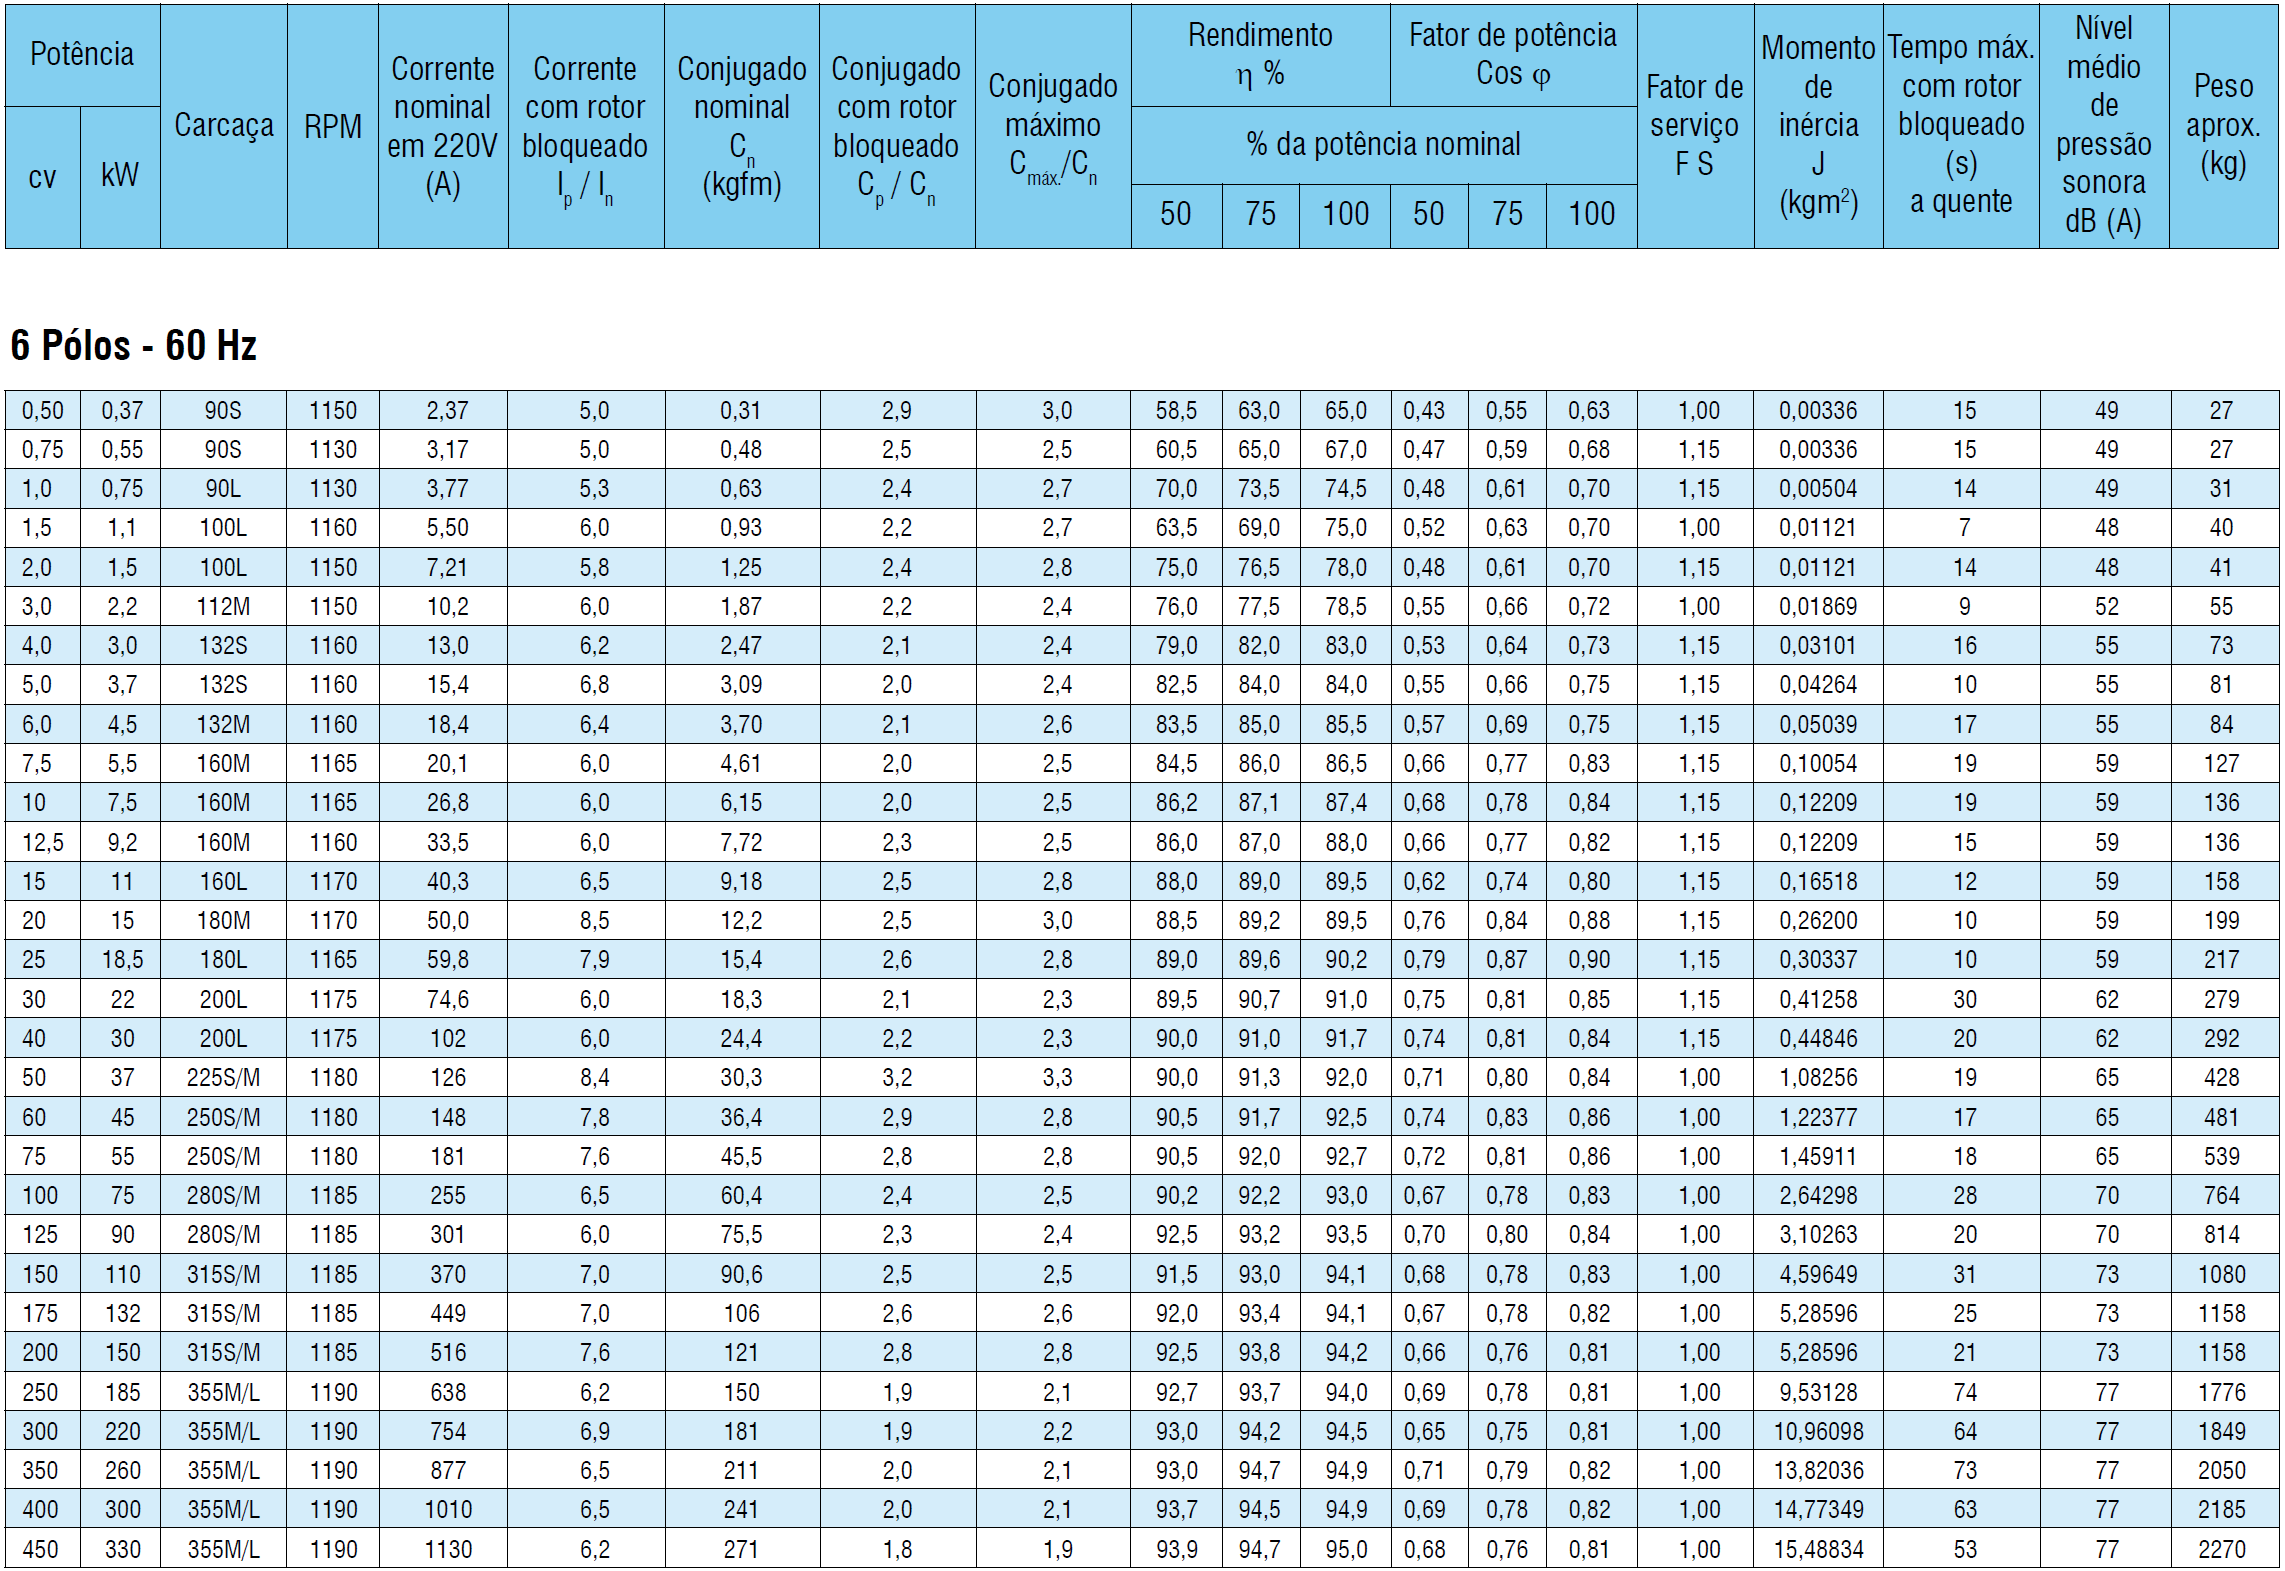
\includegraphics[width=0.8\textwidth]{content/sections/03_sistema_de_elevacao/sections/10_motor_de_elevacao/images/motor_catalogo.png}
  \caption{Catálogo de motores elétricos da WEG \cite{weg}}
  \label{fig:motor_catalogo}
\end{figure}

\begin{figure}[H]
  \centering
  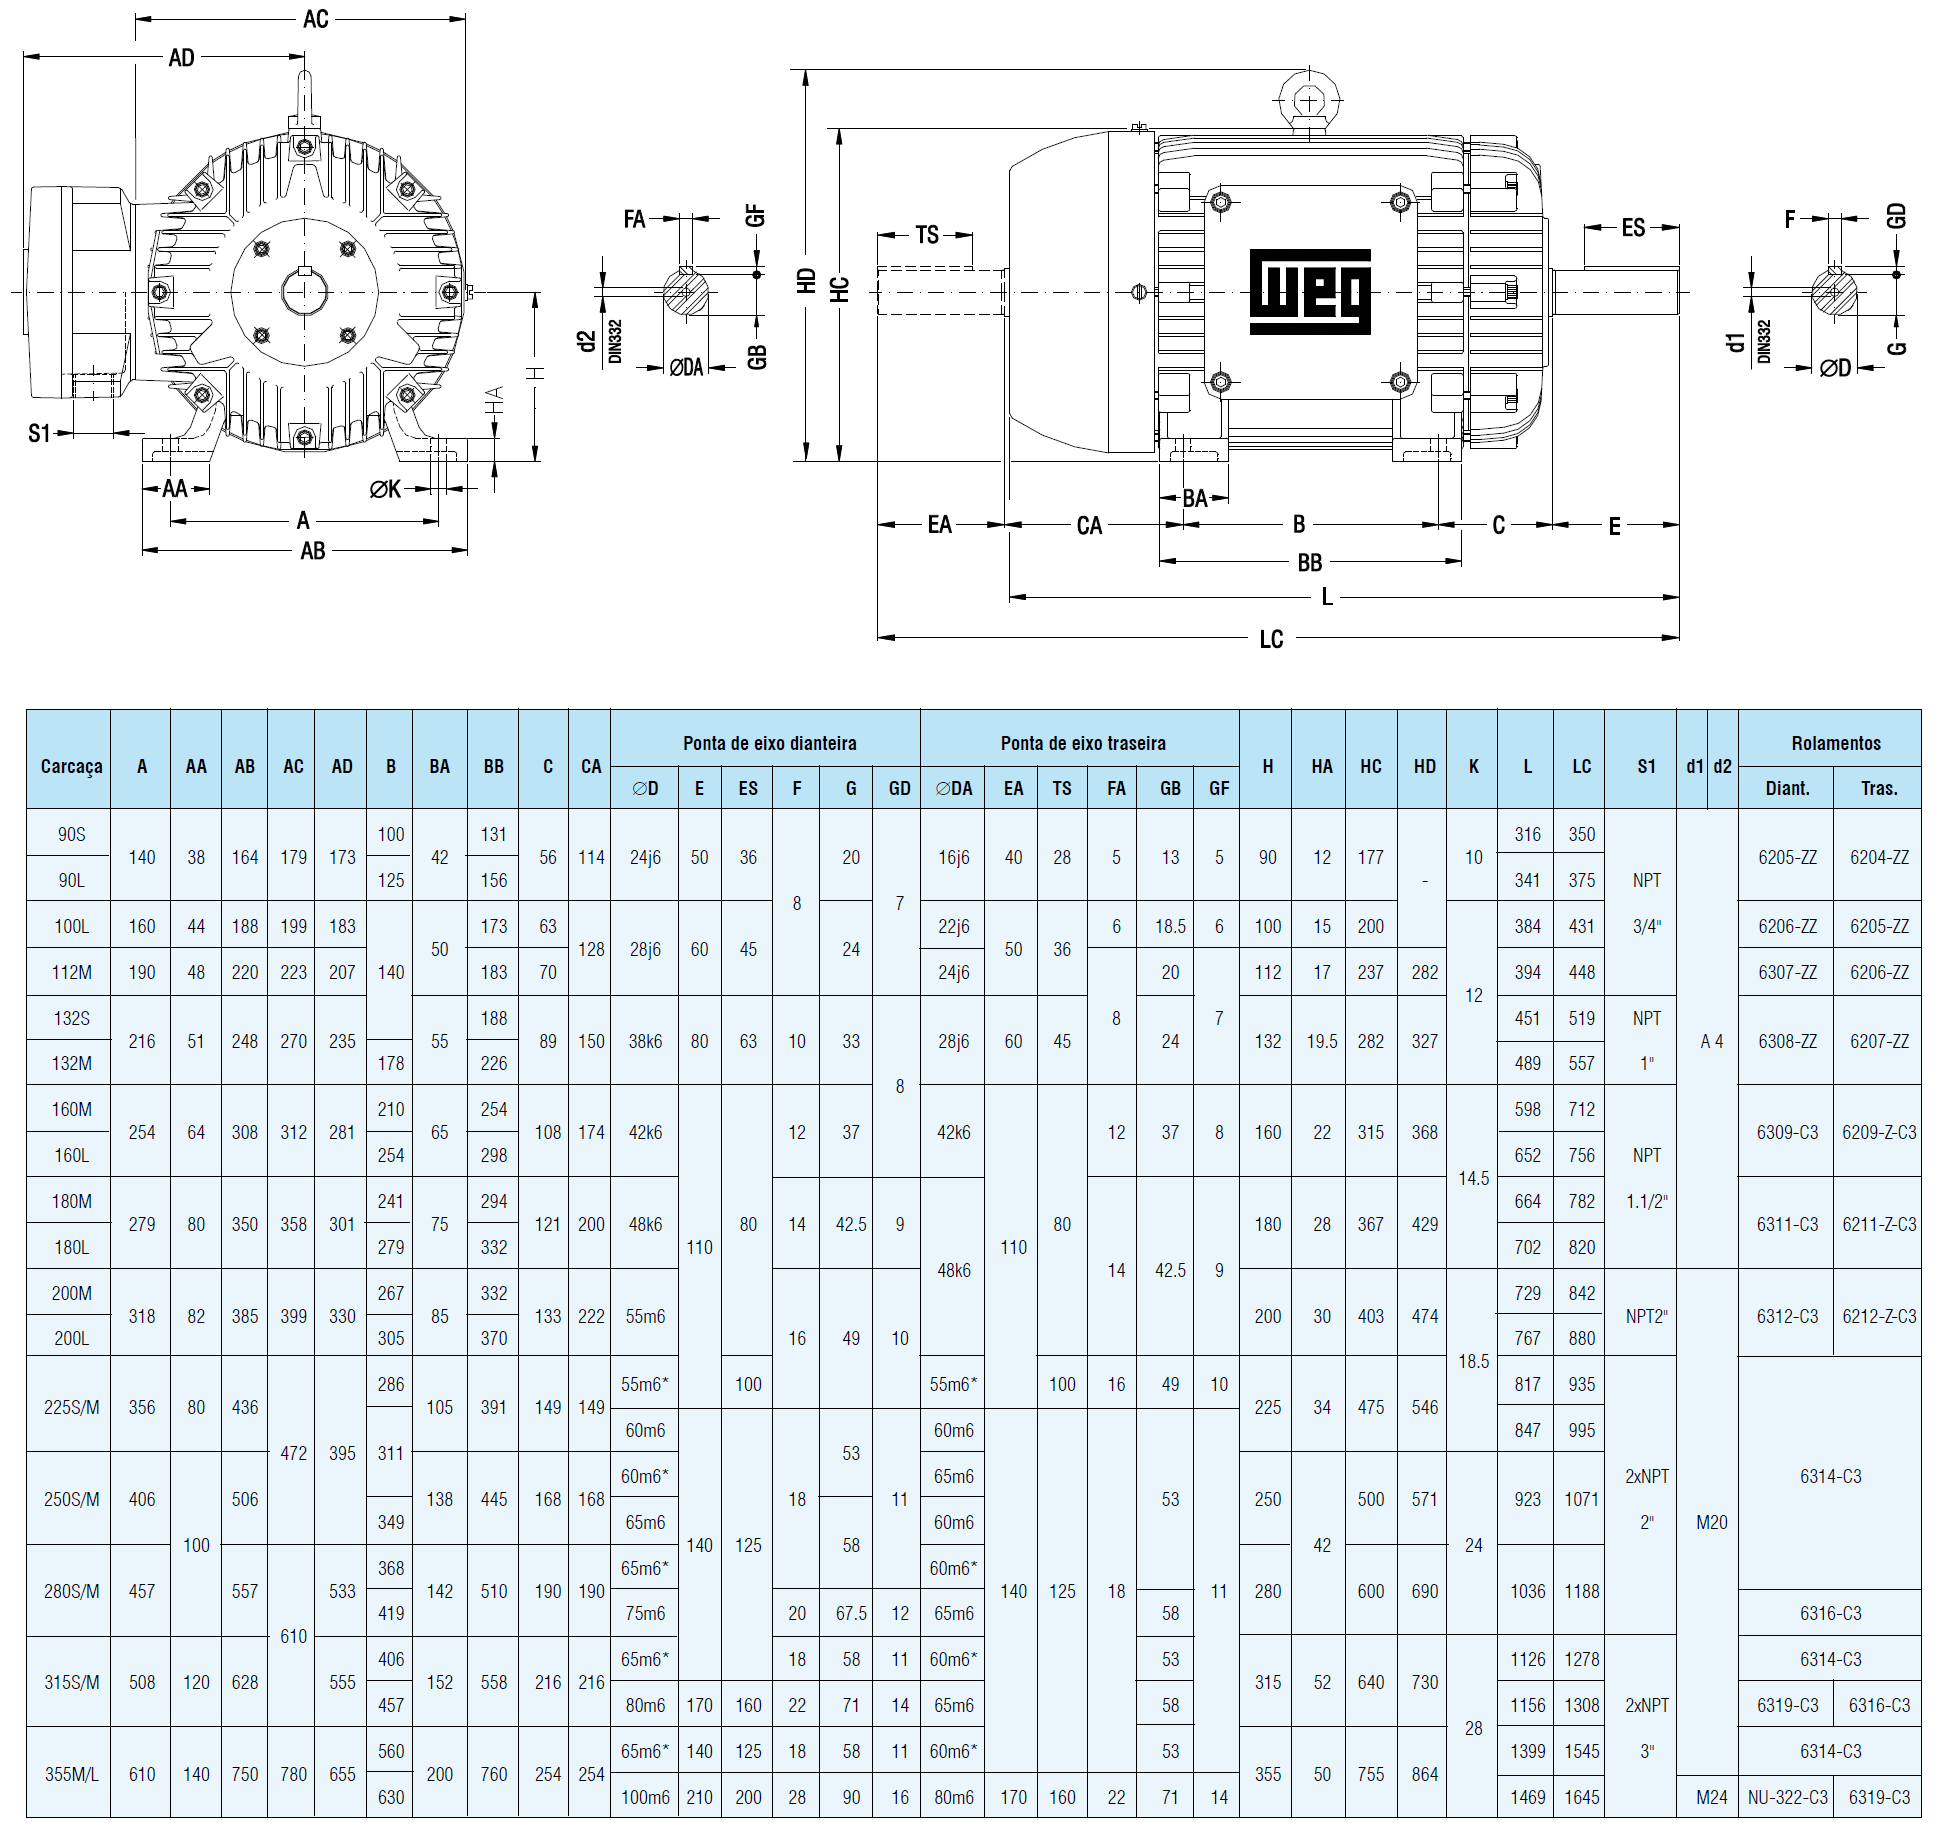
\includegraphics[width=0.8\textwidth]{content/sections/03_sistema_de_elevacao/sections/10_motor_de_elevacao/images/motor_dimensoes.png}
  \caption{Dimensões do motor adotado segundo o catálogo da WEG \cite{weg}}
  \label{fig:motor_dimensoes}
\end{figure}

\begin{table}[H]
  \centering
  \caption{Dados do motor adotado segundo o catálogo da WEG \cite{weg}}
  \begin{tabularx}{\textwidth}{>{\centering\arraybackslash}X>{\centering\arraybackslash}X>{\centering\arraybackslash}X}
    \toprule
    Descrição        & Símbolo            & Valor                 \\
    \midrule
    Potência em CV   & $N_{\text{motor}}$ & \SI{15}{\cv}          \\
    Potência em kW   & $P_{\text{motor}}$ & \SI{11}{\kilo\watt}   \\
    Rotação          & $n_{\text{motor}}$ & \SI{1170}{\rpm}       \\
    Carcaça          & -                  & 160 l                 \\
    Massa            & $M_{\text{motor}}$ & \SI{158}{\kilo\gram}  \\
    Diâmetro do eixo & $D$                & \SI{42}{\milli\meter} \\
    \bottomrule
  \end{tabularx}
\end{table}
